\chapter{Implementación}
\section{Estructura del Proyecto Django}
La estructura del proyecto sigue la convención estándar de Django, separando la configuración, la aplicación principal y los recursos estáticos y de plantillas. A continuación se muestra un diagrama UML de la organización de carpetas y archivos principales:
\begin{figure}[H]
	\centering
	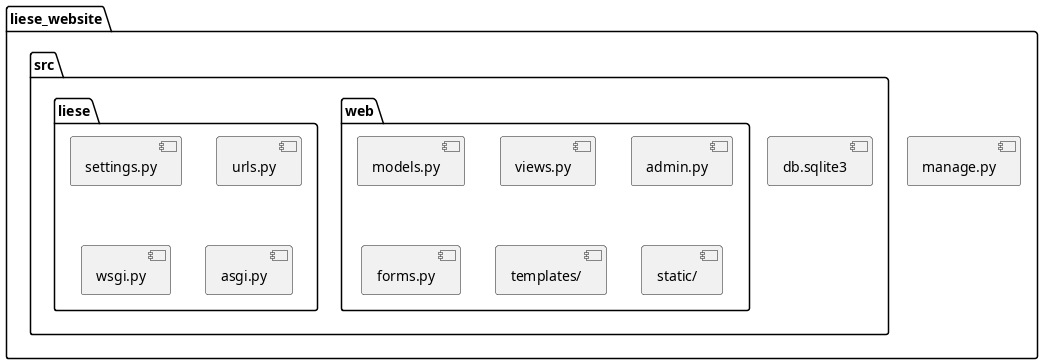
\includegraphics[width=0.9\textwidth]{uml/estructura-proyecto.png}
	\caption{Estructura de carpetas y archivos principales del proyecto Django LIESE.}
\end{figure}
\newpage
\section{Modelos, Vistas y URLs}
El flujo de interacción entre usuario, vistas y modelos se ilustra en el siguiente diagrama UML de secuencia, usando como ejemplo el proceso de solicitud de oportunidad académica:
\begin{figure}[H]
	\centering
	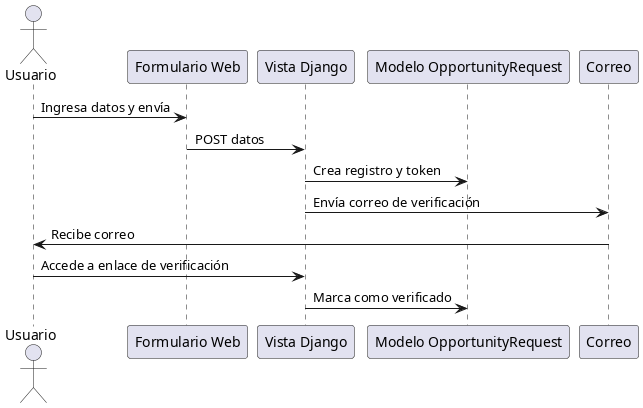
\includegraphics[width=0.95\textwidth]{uml/flujo-oportunidad.png}
	\caption{Diagrama de secuencia UML para el flujo de solicitud de oportunidad.}
\end{figure}
\section{Templates y Frontend}
El frontend utiliza el sistema de templates de Django y Bootstrap para la presentación. La herencia de plantillas y la organización de los archivos HTML ya se ilustró en el capítulo de arquitectura.
\newpage
\section{Sistema de Administración}
El panel de administración de Django permite gestionar usuarios, miembros, proyectos y contenidos. El siguiente diagrama UML de colaboración muestra la interacción entre el administrador, el panel y los modelos:
\begin{figure}[H]
	\centering
	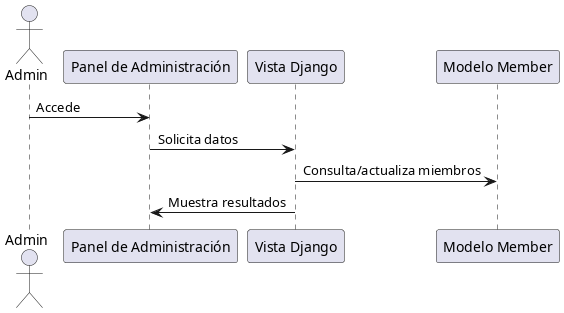
\includegraphics[width=0.7\textwidth]{uml/admin-miembros.png}
	\caption{Diagrama de colaboración UML para la administración de miembros.}
\end{figure}
